% mycsrf 'for beeing included' snippet template
%
% (c) Karsten Reincke, Frankfurt a.M. 2012, ff.
%
% This text is licensed under the Creative Commons Attribution 3.0 Germany
% License (http://creativecommons.org/licenses/by/3.0/de/): Feel free to share
% (to copy, distribute and transmit) or to remix (to adapt) it, if you respect
% how you must attribute the work in the manner specified by the author(s):
% \newline
% In an internet based reuse please link the reused parts to mycsrf.fodina.de
% and mention the original author Karsten Reincke in a suitable manner. In a
% paper-like reuse please insert a short hint to mycsrf.fodina.de and to the
% original author, Karsten Reincke, into your preface. For normal quotations
% please use the scientific standard to cite
%


%% use all entries of the bibliography

\subsection{NoteEdit ($\bigstar$)}

\parpic(1.4cm,1cm)[r][t]{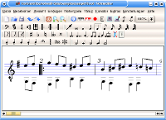
\includegraphics[width=1.4cm]{logos/noteedit-300dpi.png}}
\label{NoteEdit}Wer nach freien Notensatzprogrammen sucht, dem wird sicher auch
\acc{NoteEdit}\footcite[vgl.][\nopage wp.]{Andres2002a} vorgeschlagen. Ältere
Sichtungen gehen gern auf das Programm ein\footcite[vgl.][\nopage
wp.]{Roitman2007a}; manche mit affirmativem Ton\footcite[vgl.][\nopage
wp.]{LinuxSoundNotation2006a}, manche ohne
\footnote{\cite[vgl.][\nopage wp.]{Brendel2005a} - hier
\href{http://www.linux-magazin.de/ausgaben/2005/09/digitale-notenstecher/2/}
{http://www.linux-magazin.de/ausgaben/2005/09/digitale-notenstecher/2/} und
\texttt{\/3\/}}. Neuere Sichtungen bezeichnen es als
\enquote{obsolet}\footcite[vgl.][\nopage wp.]{WpedNotensatz2019a}.
Der Quellcode des Programms ist allerdings auch heute noch
erreichbar\footnote{\cite[vgl.][\nopage wp.]{NoteeditRep2014a}. Das Repository sagt,
das Programm stünde unter der GPL-2.0 Lizenz. Damit wäre es freie Software.},
eine ausführbare Version wird in der Regel aber nicht mehr angeboten, weder im
Netz, noch als Distri\-bu\-tions\-paket\footnote{jedenfalls nicht in Ubuntu
18.04.}. Gelegentlich wird erwähnt, dass spätere Entwickler von \acc{Noteedit}
schließlich zu \acc{Canorus} gewechselt seien\footnote{$\rightarrow$
\href{https://wiki.ubuntuusers.de/Canorus/}{https://wiki.ubuntuusers.de/Canorus/}
} und dass \acc{Canorus} nun der \enquote{offizielle Nachfolger} von
\acc{Noteedit} sei\footcite[vgl.][\nopage wp.]{WpedCanorus2019a}.
Jedenfalls verlinkt auch sein ursprünglicher Autor \acc{NoteEdit} in seiner Vita
auf eine Homepage, die nicht mehr erreichbar ist\footnote{Offensichtlich ist
Notedit zunächst auf dem deutschen FOSS-Repository \acc{Berlios} gehostet worden
und nach dessen Einstellung nach Sourceforge migriert worden. An der Verlinkung
kann man das noch erkennen. \cite[vgl. dazu][\nopage wp.]{Andres2018a}.}.

Dass der Quelltext noch zugänglich
ist\footcite[vgl.][\nopage wp.]{NoteeditRep2014a}, löst das Problem nicht. Zwar
gehören zum Paket auch die Installationsskripte. Aber diese fordern Komponenten an,
die heute ob ihres Alters nicht mehr (so einfach) zur Verfügung stehen. Eine
direkte Installation aus den Quellen heraus misslingt also. So bleibt nur der
Schluss, dass dieses Programm vorerst nicht mehr nutzbar ist\footnote{Gleichwohl
werden die Quellen samt der GNU-make-Files ausgeliefert. Damit steht einer
Aktualisierung prinzipiell nichts im Wege. Es ist 'nur' eine Frage des
Programmier- und Konfigurationsaufwandes, bis \acc{NoteEdit} über die Aufrufe
\texttt{autoconf automake configure --prefix=/dir make make install} wieder zur
Verfügung stünde. Ob sich solch eine 'Wiederbelebung' lohnt, ist letztlich eine
Frage der Lust am Programmieren, nicht der Lust am Musizieren. }. Das ist
insofern bedauerlich, als es eines der wenigen Programme (gewesen) sein soll,
die ihren Inhalt auch als MusiX\TeX-Datei exportieren
konnten\footcite[vgl.][\nopage wp.]{Roitman2007a}.

Wir geben \acc{NoteEdit} also 1 von 5 Sternen. Denn in der Vergangenheit hat das
Programm wesentlich zum Komponieren und Arrangieren mit freier Software
ermuntert.


% this is only inserted to eject fault messages in texlipse
%\bibliography{../bib/literature}
